\documentclass[11pt]{jsarticle}

% パッケージの宣言
\usepackage{url}
\usepackage{here}
\usepackage{natbib}
\usepackage{color}
\usepackage[dvipdfmx]{graphicx}
\usepackage{amsmath}
\usepackage{amsfonts}
\usepackage{amssymb}
\usepackage{bm}
\usepackage{multirow}
%\usepackage{tabudlarx}
\usepackage{latexsym}

%argmax,argmin の定義
\DeclareMathOperator*{\argmin}{arg\,min}
\DeclareMathOperator*{\argmax}{arg\,max}



\title{hoge}
\author{foo \thanks{aaa} \and bar \thanks{bbb}}

\begin{document}

\maketitle

 \thispagestyle{empty}

\begin{abstract}
要旨を書く。
\end{abstract}

\begin{center}
キーワード:条件付きプロビットモデル、階層ベイズモデル、ブランドロイヤルティ、\\ みたいなかんじで書く

\end{center}

\newpage

\pagenumbering{roman} % 目次はローマ数字
 \setcounter{page}{1}

\tableofcontents

\newpage
\pagenumbering{arabic}
 \setcounter{page}{1}


% ここから本文

\section{ABC}
この章では。。。

\subsection{abc}
参考文献は「\citet{rosenbaum1983central}によると」のように書く

また、数式は equation 環境を使う

\begin{equation}
 \alpha + \beta = \gamma
\end{equation}

ここで、以下のようにラベルをつけると式(\ref{eq:indicator1})のように本文中で参照できる

\begin{equation} \label{eq:indicator1}
y_k^i(n) = \begin{cases}
             1 \;\; if \; \mbox{$n$回目の消費者$i$の$k$の選択}\\ % 式の中で日本語を使うときは mbox
             0 \;\; if \; otherwise
             \end{cases}
\end{equation}


\subsection{aabbcc}
複数行の式は align 環境。

例: ロジットの IIA 問題

\begin{align} \label{eq:teruilogit}
Pr(y_{it}=A) &= \frac{\exp(p_{Ait} \beta)} {\exp(p_{Ait} \beta) + \exp(p_{Bit} \beta)} \\ % 改行, &で位置を揃える
\nonumber Pr(y_{it}=B) &= \frac{\exp(p_{Bit} \beta)} {\exp(p_{Ait} \beta) + \exp(p_{Bit} \beta)} % 式番号をつけたくないときは手前に nonumber
\end{align}
となる。オッズ比は

\begin{equation} \label{eq:teruilogit2}
  \frac {Pr(y_{it}=A) } {Pr(y_{it}=B)} = \frac {\exp(p_{Ait} \beta)} {\exp(p_{Bit} \beta)}
\end{equation}
と書けるが、これに選択肢 C が追加された場合、

\begin{align} \label{eq:teruilogit3}
Pr(y_{it}=A) &= \frac{\exp(p_{Ait} \beta)} {\exp(p_{Ait} \beta) + \exp(p_{Bit} \beta) + \exp(p_{Cit} \beta)} \\
Pr(y_{it}=B) &= \frac{\exp(p_{Bit} \beta)} {\exp(p_{Ait} \beta) + \exp(p_{Bit} \beta) + \exp(p_{Cit} \beta)}
\end{align}
と変化するが、オッズ比は(\ref{eq:teruilogit2})のままである。すなわち、選択肢の数が変化したにも関わらず、選択確率は一定であり、一般的な消費者行動と一致しない。
また、統計的操作性から誤差項がガンベル分布に従うとするよりも、正規分布に従うとするほうが現実の消費者像に近いと言える。すなわち、多項ロジットモデルを利用

\section{DEF}
\subsection{箇条書き}

\begin{itemize}
 \item aaa
 \item bbb
 \item kkk
 \item lll
\end{itemize}

\begin{enumerate}
 \item lll
 \item alk
\end{enumerate}

\subsection{画像}
\begin{figure}[htbp] % htbp は位置の指定。特別なことがなければこれでよい
 \centering
 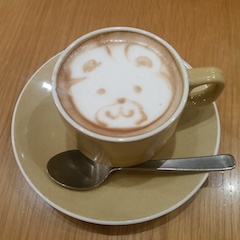
\includegraphics[width=5cm]{./img/favicon.png}
  \caption{匿名知的集団ホクソエム}
  \label{fig:favicon}
\end{figure}

\subsection{表}
頑張って書いてもいいけど、Excel から Web(http://rra.yahansugi.com/scriptapplet/csv2tabular/index.html)で変換して原型を作り、枠線だけ付け加えるのがよい。


\begin{table}[htbp]
  \centering
  \caption{論点の整理}
 \begin{tabular}{c|c|c}
  1 & 2 & 3 \\ \hline
  4 & 5 & 6 \\
  7 & 8 & 9
 \end{tabular}
\end{table}

\section{その他}
各自調べてください。


\newpage
\appendix % 付録開始
\section{MCMC アルゴリズム}

\section{おまけの図表とか}

\newpage

\bibliographystyle{jecon}
\bibliography{sample}


\end{document}

